\section{Background}\label{MPC}
This section gives a brief overview of three topics important for understanding the problem being addressed: state space models, model predictive optimal control, and the splitting method.
\subsection{State Space Model}
In our paper, MPC is based on a state space model of a physical system. A discrete state-space model defines what state a system will be in one-time step into the future, based on the current state of the system and current input acting upon it. A generic linearized discrete state-space system model consists of matrices A, B, C, and D\footnote{it is common to omit the matrix D, as inputs typically do not directly impact output} and is formulated as follows:

\begin{equation}
\label{eq:xk}
x_{k+1}=A x_k + B u_k 
\end{equation}  
\begin{equation}
\label{eq:yk}
y_{k}=C x_k + D u_k  
\end{equation}  

Where:
\begin{itemize}
  \item $x_k$ represents the state of the system at time $k$
  \item $u_k$ represents the input acting on the system at time $k$
  \item $y_k$ represents outputs of the system at time $k$
  \item $A$ is a matrix that defines the internal dynamics of the system
  \item $B$ is a matrix that defines how the input acting upon the system impact its state
  \item $C$ is a matrix that transforms states of the system into outputs ($y_k$)
\end{itemize}

Equation\cref{eq:xk} is referred to as the state update equation. With respect to a closed loop control system, matrix $A$ represents the dynamics of the plant being controlled, matrix $B$ represents how actuator commands (i.e. $u_k$) impact the plant, and the matrix $C$ could be viewed as a mapping of the current state to the output obtained from sensors (i.e. $y_{k}$).

Also the width (i.e. number of columns) of each matrix or length of each vector found in Equation\cref{eq:xk} and \cref{eq:yk} can be viewed as follows:
\begin{itemize}
  \item $M$: the number of system/plant inputs/actuators.
  \item $N$: the number of system/plant states.
  \item $P$: the number of system outputs (i.e. sensors). 
  \item $A \in \mathbb{R}^{N\times N}$; $B \in \mathbb{R}^{N\times M}$; $C \in \mathbb{R}^{P\times N}$.
  \item $x_{k} \in \mathbb{R}^{N}$; $y_k \in \mathbb{R}^{P}$; $u_k \in \mathbb{R}^{M}$.
\end{itemize}


\subsection{Model Predictive Optimal Control}
MPC uses Equation\cref{eq:xk,eq:yk} to predict the behavior of the system from current time over a future prediction horizon, thus the input ($u_k$), input-change rate/step ($\Delta u_k$) and state ($x_k$) are augmented to cover future predictions, as in Formula\cref{eq:aug}.

\begin{equation}
\scalemath{0.8}{
U_k=
\begin{bmatrix}
u_k\\
u_{k+1}\\
\vdots \\
u_{k+H_u}
\end{bmatrix}
\text{,}\quad
\Delta U_k=
\begin{bmatrix}
\Delta u_k\\
\Delta u_{k+1}\\
\vdots \\
\Delta u_{k+H_{u-1}}
\end{bmatrix}
\text{,}\quad
X_k=
\begin{bmatrix}
x_k\\
x_{k+1}\\
\vdots \\
x_{k+H_p}
\end{bmatrix}\label{eq:aug}}
\end{equation}
Where:
\begin{itemize}
	\item $H_u$: changeable future input horizon. We assume input $u_k$ will be constant after $H_u$ time steps.
	\item $H_p$: prediction horizon. Normally, $H_p\geq H_u$. 
	\item $U_k \in \mathbb{R}^{M(H_{u}+1)}$, $\Delta U_k \in \mathbb{R}^{MH_{u}}$, $X_k \in \mathbb{R}^{N(H_{p}+1)}$.
\end{itemize}\par
\subsubsection{MPC Cost Function}
An MPC controller specifies a vector combination of all controlled variables($X_k$) and constraint variables($\Delta U_k$, $U_k$), which minimizes the quadratic objective cost function given by Equation\cref{eq:costf}, subject to linear constraints on the variables $x_i$, $u_i$ and $\Delta u_i$. $q_i$, $p_i$ and $s_i$ are positive cost constant applied to $x_i$, $u_i$ and $\Delta u_i$.
\begin{equation}
\begin{split}
\mathbb{C}(k)=\frac{1}{2}\Big( \sum_{i=k}^{k+H_p}(x_i^Tq_ix_i-2r_i^Tq_ix_i)+\sum_{i=k}^{k+H_u}u_i^Tp_iu_i\\
+\sum_{i=k}^{k+H_{u-1}}\Delta u_i^Ts_i\Delta u_i\Big)+Const
\label{eq:costf}
\end{split}
\end{equation}
Where $r_k$ is a proposed trajectory at time $k$. Since the optimal solution is independent of $Const$, we omit this constant term and rewrite the cost function into more condense format:
\begin{equation}
\mathbb{C}(k)=\frac{1}{2}
\begin{bmatrix}
X_k\\
U_k\\
\Delta U_k
\end{bmatrix}^T
\begin{bmatrix}
Q& & \\
 &P& \\
& &S 
\end{bmatrix}
\begin{bmatrix}
X_k\\
U_k\\
\Delta U_k
\end{bmatrix}
-
R_k^TQX_k
\end{equation}
Where $R_k$ is the vector augmented form of $r_k$, and has the same format and size as $X_k$. The $Q$ matrix is shown in\cref{eq:costconst} and the same format applies to the $P$ and $S$ matrix.

\subsubsection{Constraints}
The equality constraints are associated with the system time-step update, which is written as Equation\cref{eq:quad}. It contains the augmented form of Equation\cref{eq:xk} and\cref{eq:yk} and the equality relationship between $U_k$ and $\Delta U_k$. The inequalities are the restrictions on $U_k$, $\Delta U_k$ and $X_k$. Normally, the constraints to the state and input are called the box constraint, which sets a low boundary and a high boundary like an enclosed box that circumscribes the scope of these variables.

\subsection{Splitting Method}
One technique for partitioning variables in ADMM is writing the convex QP problem into consensus form~\cite{6422363}:
\begin{align*}
&minimize:\;  \mathbbm{1}_{\mathcal{D}}(\chi)+\phi(\chi) +\mathbbm{1}_{\mathcal{C}}(\zeta)\\
 &subject\;  to:\; \chi=\zeta
\numberthis \label{eq:split}
\end{align*}
Where $\mathbbm{1}_{\mathcal{D}}(\chi)$ is the indicator function: $\mathbbm{1}_{\mathcal{D}}:\chi\rightarrow \{ 0,+\infty \}$. $\mathcal{D}$ is the affine set associated with system update in Equation \cref{eq:quad}. When $\chi$ fails to meet the equality condition,  $\mathbbm{1}_{\mathcal{D}}(\chi)$ goes infinity. So does $\mathbbm{1}_{\mathcal{C}}(\zeta)$, where $\mathcal{C}$ is the variable constraints that the system must comply.\par
We use function $f+g$ to replace the objective function in QP problem\cref{eq:split}. $f$ and $g$ are shown in in Equation\cref{eq:gf}. Starting from arbitrary points $\zeta^0$ and $\upsilon^0$, the operator splitting method solves the QP problem by carrying out three steps:\cref{eq:xi,eq:zi,eq:vi} repeatedly. Each can be solved separately without division.
%Operator splitting method decomposes Formula\cref{eq:split} QP problem into three computating steps: Equation\cref{eq:xi},\cref{eq:zi} and\cref{eq:vi}. Each can be solved seperately without division. 
%\begin{equation}
%\underset{v}{\max}\;\underset{z,x}{\inf}L_p(z,x,v):\;  I_{\mathcal{D}}(x)+\phi(x) +\psi(z)+v^T(x-z)\\
%\end{equation}

%\begin{align}
%&x_{i+1}:=arg\;\underset{x}{\min}L_{\rho}(z_i,x,v_i)\\
%&z_{i+1}:=arg\;\underset{z}{\min}L_{\rho}(z,x_{i+1},v_i)\\
%&v_{i+1}:=v_i+\rho (x_{i+1}-z_{i+1})
%\end{align}

\begin{align*}
&g(\chi)=\mathbbm{1}_{\mathcal{D}}(\chi)+\phi(\chi)\\
&f(\zeta)=\mathbbm{1}_{\mathcal{C}}(\zeta) 
\numberthis \label{eq:gf}
\end{align*}
%\begin{align*}
%&x^{i+1}:=prox_{g,\rho}(z^i+v^i)\\
%&z^{i+1}:=prox_{f,\rho}(x^{i+1}+v^i)\\
%&v^{i+1}:=v^i+\rho (x^{i+1}-z^{i+1})
%\numberthis \label{eq:prox}
%\end{align*}
\begin{align}
&\chi^{i+1}:=prox_{g,\rho}(\zeta^i+\upsilon^i)\label{eq:xi}\\
&\zeta^{i+1}:=prox_{f,\rho}(\chi^{i+1}+\upsilon^i)\label{eq:zi}\\
&\upsilon^{i+1}:=\upsilon^i+\rho (\chi^{i+1}-\zeta^{i+1})\label{eq:vi}
\end{align}
Here, $i$ is the iteration counter, $prox_{f,\rho}(\chi)$ is the proximal mapping (or proximal operator) of a convex function $f$: 
\begin{equation*}
prox_{f,\rho}(\chi)=arg\;\underset{u}{\min}(f(u)+\frac{\rho}{2}\| \chi-u\| _2^2)
\end{equation*}
$\rho>0$ is the dual update step length. 

Computing $\chi^{i+1}$ in\cref{eq:xi} is equivalent to solving $\chi^{i+1}$ in\cref{eq:quad}, which is the standard QP problem with equality constraints. 
\begin{align*}
&minimize:\;  \frac{1}{2} ({\chi^{i+1}})^{T}E\chi^{i+1}+l^T\chi^{i+1}\\
 &subject\;  to:\; G\chi^{i+1}=h
\numberthis \label{eq:quad}
\end{align*}

The associated matrices/vectors are shown in Equation\cref{eq:g,eq:omega,eq:costconst}:
\setcounter{MaxMatrixCols}{20}
\begin{equation}
\arraycolsep=3pt
\scalemath{0.8}{
G=
}
\scalemath{0.6}{
\begin{bmatrix}
   I & \dots & \dots & \dots  & \dots &\dots & \dots & \dots &\dots &\dots & \dots & \dots&\dots &\dots & \dots & \dots\\
   A & -I & \dots & \dots  & \dots & \dots & B & \dots & \dots &\dots &\dots & \dots & \dots &\dots &\dots & \dots\\
	\dots & A & -I & \dots & \dots & \dots& \dots&B& \dots &\dots &\dots & \dots & \dots &\dots &\dots & \dots\\
	\dots & \dots  & \dots & \dots & \dots & \dots  & \dots &\dots &\dots & \dots & \dots &B & \dots &\dots &\dots & \dots\\
\vdots & \vdots & \vdots & \vdots & \vdots & \vdots  & \vdots & \vdots  & \vdots & \vdots & \vdots & \vdots  & \vdots & \vdots & \vdots & \vdots\\
\dots & \dots & \dots & \dots & A & -I & \dots & \dots & \dots & \dots & \dots & B & \dots &\dots &\dots & \dots\\
\dots & \dots & \dots & \dots & \dots & \dots & I & -I & \dots & \dots & \dots & \dots & I & \dots  & \dots  & \dots\\ 
\dots & \dots & \dots & \dots & \dots & \dots &\dots  & I & -I & \dots & \dots & \dots & \dots & I  & \dots & \dots\\
\vdots & \vdots & \vdots & \vdots & \vdots & \vdots  & \vdots & \vdots  & \vdots & \vdots & \vdots & \vdots  & \vdots & \vdots & \vdots & \vdots\\
\dots & \dots & \dots & \dots & \dots & \dots &\dots  &\dots &\dots &\dots & I & -I &\dots & \dots & \dots & I
\end{bmatrix}}
\label{eq:g}
\end{equation}

\begin{equation}
\chi^{i+1}=
\scalemath{0.7}{
\begin{bmatrix}
  x_k\\
	x_{k+1}\\
	x_{k+2}\\
   \vdots\\
	x_{k+H_p}\\
u_{k}\\
u_{k+1}\\
\vdots\\
u_{k+H_u}\\
\Delta u_{k}\\
\Delta u_{k+1}\\
\vdots\\
\Delta u_{k+H_u-1}
\end{bmatrix}
\label{eq:omega}
\text{,}\quad
h=
\begin{bmatrix}
x_{k}\\
0\\
\vdots\\
0
\end{bmatrix}
\text{and}\quad
l=
\begin{bmatrix}
	Q*R_k\\
	\textbf{0}_{(2H_u+1)M}
\end{bmatrix}-
\rho \begin{bmatrix}
\zeta_0^i+\upsilon_0^i\\
\zeta_1^i+\upsilon_1^i\\
\vdots\\
\zeta_{S2-1}^i+\upsilon_{S2-1}^i
\end{bmatrix}}
\end{equation}
%f=
%\begin{bmatrix}
%q_0^Tr_0-\rho (z_0^k+v_0^k) \\
%q_1^Tr_1-\rho (z_1^k+v_1^k) \\
%\vdots\\
%q_{H_p}^Tr_{H_p}-\rho (z_{H_p}^k+v_{H_p}^k)\\
%0-\rho (z_{H_p+1}^k+v_{H_p+1}^k)\\
%\vdots\\
%0-\rho (z_{S2-1}^k+v_{S2-1}^k)
%\end{bmatrix}}
%\end{equation}
%%%%%%%%%%%%%%%%%%%%%%%%%%%%%%%%%%%%%%%%%%%%%%%

%%%%%%%%%%%%%%%%%%%%%%%%%%%%%%%%%%%%%%%%%%%%%%%
\begin{equation}
\scalemath{0.7}{
E=
\begin{bmatrix}
Q+\rho I& & \\
 &P+\rho I& \\
& &S+\rho I 
\end{bmatrix}
\quad\text{and}\quad
Q=
\begin{bmatrix}
q_0&&&\\
&q_1&&\\
&&\ddots&\\
&&&q_{H_p} 
\end{bmatrix}}
\label{eq:costconst}
\end{equation}

Let $S_1=(H_p+1)N+H_uM$, and the number of optimization variables $S_2=(H_p+1)N+(2H_u+1)M$, then $G \in \mathbb{R}^{S_1\times S_2}$, $E \in \mathbb{S}_{+}^{S_2\times S_2}$.

The common method to solve Equation\cref{eq:quad} is to establish the KKT condition. The KKT condition is shown below:
\begin{equation}
\begin{bmatrix}
E&G^T\\
G&\textbf{0} 
\end{bmatrix}
\begin{bmatrix}
\chi^{i+1} \\
\lambda 
\end{bmatrix}=
\begin{bmatrix}
-l\\
h
\end{bmatrix}
\label{eq:kkt}
\end{equation}
Where $\lambda$ is called the dual variable vector. $E$ is the diagonal combination of cost constant matrix $Q$, $P$ and $S$ as is shown in Equation\cref{eq:costconst}. The KKT matrix is proved to be invertible\cite{6422363}.

We solve Equation\cref{eq:kkt} to obtain $\chi^{i+1}$, which gives:
\begin{equation}
\begin{bmatrix}
\chi^{i+1} \\
\lambda 
\end{bmatrix}=
\begin{bmatrix}
E&G^T\\
G&\textbf{0} 
\end{bmatrix}^{-1}
\begin{bmatrix}
-l\\
h
\end{bmatrix}
\label{eq:sol}
\end{equation}

The KKT matrix is nonsingular. We use the following matrix $M$ to represent the inverse of the KKT matrix:
\begin{equation*}
\begin{bmatrix}
M_{11}&M_{12}\\
M_{12}^T&M_{22} 
\end{bmatrix}
=
\begin{bmatrix}
E&G^T\\
G&\textbf{0} 
\end{bmatrix}^{-1}
\end{equation*}
%Where $	\begin{bmatrix}
%	M_{11}&M_{12}
%	\end{bmatrix}\in \mathbb{R}^{S_2 \times (S_1+S_2)}$. 
Where $M_{11} \in \mathbb{R}^{S_2 \times (S_2+N)}$. We do not care about matrix $M_{12}$ and $M_{22}$ because $M_{12}$ will multiply with a \textbf{0} vector ($h$ vector is constituted by $x_{k}$ and zero elements) and $M_{22}$ produces the result of the dual variable $\lambda$, which is only required when constructing the KKT condition. In this way, only $M_{11}$ is useful in our computation. This formulation of constructing the MPC formula reduces to the orignal storage requirement by $\frac{S1+S2}{S1-N}$, which is by $42.82\%$ in the mass-spring system example in \cref{eva}.

%According to\cite{6422363}, there is an approach to solve Equation\cref{eq:kkt} through sparse $LDL^T$ decomposition. $LDL^T$ decomposition method can reduce the complexity of the factor and solve steps if we exploit additional sparsity of these matrices. In the future, we will explore a hardware solution considering such as decomposition method. Currently, for the simplicity of the hardware dataflow pipeline design, we use a dense matrix computation solution of Equation\cref{eq:sol} solution.

%The solution to\cref{eq:zi} is the result of a saturation function. The saturation algorithm is shown in algorithm\cref{alg:sat}, where $\textbf{dom}\: \mathcal{C}$ is the feasible interval of vector $\omega$. 
%\begin{algorithm}
%  \uIf{$x \in \textbf{dom}\: {\mathcal{C}}$}{
%    return $x$\;
%  }
%  \uElse{
%    return nearest boundry/constraint value of $\textbf{dom}\: \mathcal{C}$\;
%  }
%\caption{Saturation Function: $sat(x,\textbf{dom}\: {\mathcal{C}})$}\label{alg:sat}
%\end{algorithm}

%We summarize the splitting method in Fig.\cref{fig:dataflow} step by step, where step 1$\sim$3 correspond with operations\cref{eq:xi,eq:zi,eq:vi} respectively.
%\begin{figure}[!ht]
%\centering
%\captionsetup{justification=centering}
%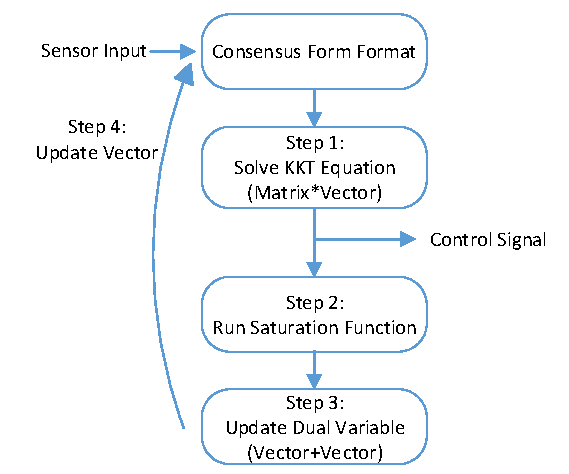
\includegraphics[scale=.75]{../figure/dataFlow.pdf}
%\DeclareGraphicsExtensions.
%\caption{MPC Control Dataflow using ADMM\label{fig:dataflow}}
%\end{figure}

The solution to\cref{eq:zi} is the result of a saturation function. The detailed processing steps are shown in Algorithm\cref{alg:ADMM}, which is pipelined in hardware. A common stopping criteria is to check if $\lVert \zeta^{i+1}-\zeta^i\rVert$ or $\lVert \upsilon^{i+1}-\upsilon^i\rVert$ is smaller than a certain value. We instead use a fixed number of iterations as the stopping criteria since for many control applications a relatively small number of iterations provides sufficient controller accuracy \cite{6422363}, and this reduces hardware complexity.

\begin{algorithm}
Start from $i=0$ with arbitrary $\zeta^0$ and $\upsilon^0$.
\SetKwRepeat{Do}{do}{until}
\caption{ADMM algorithm}\label{alg:ADMM}
\Do{stopping criterion is satisfied}{
$l:=
\begin{bmatrix}
	Q*R_k\\
	\textbf{0}
\end{bmatrix}-\rho (\zeta^{i}+\upsilon^{i})$   \tcp{Update Vector l}
	$\chi^{i+1}:=
	M_{11}*
	\begin{bmatrix}
	-l&x_{k}
	\end{bmatrix}^T$ \tcp{Solve KKT}
	$\zeta^{i+1}:=sat(\chi^{i+1}-\upsilon^i,\textbf{dom}\: {\mathcal{C}})$   \tcp{Saturation}
	$\upsilon^{i+1}:=\upsilon^i+\rho (\zeta^{i+1}-\chi^{i+1})$   \tcp{Update Dual}
	$i:=i+1$
}
\end{algorithm}

As a final note on Algorithm\cref{alg:ADMM}, the $\chi^{i+1}$ appearing in line 5 and 6 is substituted with $\alpha \chi^{i+1}+(1-\alpha )\zeta^{i}$.
%\begin{equation}
%\label{eq:re}
%\alpha x^{i+1}+(1-\alpha )z^{i}
%\end{equation}
$\alpha \in (0,2)$ is the relaxation parameter derived from Douglas-Rachford splitting. The convergence rate can be improved if $\alpha$ is properly selected. %For more details about relaxation parameter refer to\cite{Eckstein92onthe}.